\documentclass{article}
\usepackage{../fasy-hw}
\usepackage{hyperref}
\usepackage{algpseudocode}
\usepackage{graphicx}

%% UPDATE these variables:
\renewcommand{\hwnum}{0}
\title{Advanced Algorithms, Homework \hwnum}
\author{Sarah Montalbano}
\collab{No Collaborators}
\date{due: 30 August 2021}

\begin{document}

\maketitle

This homework assignment should be
submitted as a single PDF file both to D2L and to Gradescope.

General homework expectations:
\begin{itemize}
    \item Homework should be typeset using LaTex.
    \item Answers should be in complete sentences and proofread.
    \item You will not plagiarize, nor will you share your written solutions
        with classmates.
    \item List collaborators at the start of each question using the
        \texttt{collab} command.
    \item Put your answers where the \texttt{todo} command currently is (and
        remove the \texttt{todo}, but not the word \texttt{Answer}).
\end{itemize}

%%%%%%%%%%%%%%%%%%%%%%%%%%%%%%%%%%%%%%%%%%%%%%%%%%%%%%%%%%%%%%%%%%%%%%%%%%%%%%
\collab{N/A}
\nextprob{Getting to Know You}

Answer the following questions:
\begin{enumerate}
    \item What is your elevator pitch?  Describe yourself in 1-2
                sentences.

        \paragraph{Answer}{I'm using my quantitative skills to produce original policy research that supports the ideals of liberty and freedom for all. In my career, I intend to analyze data, articulate both data and philosophic principles together, and use my CS skills to provide technical support for the organizations I work for.}

     \item What was your favorite CS class so far, and why?

         \paragraph{Answer}{I always enjoy classes that rely more heavily on language rather than programming. For that reason, I enjoyed Discrete Structures (Spring 2019). I'm intrigued by philosophic logic, and I found Discrete Structures to align with that interest. I enjoyed Human Computer Interaction last semester, more than most CS classes, chiefly because the subject matter was directly applicable to real life, but also because the assignments were long-form essays that I could elaborate on as much as I'd like.}

     \item What was your least favorite CS class so far, and why?

         \paragraph{Answer}{My least favorite class was Data Structures and Algorithms (232) because it relied so much on implementation and coding. The mathematical logic behind the algorithms were tough to grasp based on lecturing alone, but it was tougher to actually go home and struggle to implement the algorithms.} 

     \item Why are you interested in taking this course?

         \paragraph{Answer}{I'm fascinated by logic, in any fields I encounter. I want to know why things work and learn how to prove it.} 

     \item What is your biggest academic or research goal for this semester (can
         be related to this course or not)?

         \paragraph{Answer}{My classes this semester are entirely computer science, except Graphical \& Statistical Computing, and it is likely the hardest workload I'm going to have. Thus, I hope to maintain As and an occasional B in all of my courses in order to keep my scholarship. I am excited for Computational Biology, as I used to want to go into that field. Aside from academics, I have a large data science project for work that I have been organizing over the last 2 years, and it needs to be finished by December; that's a tall order, but should be doable with the skills I'm learning.} 

     \item What do you want to do after you graduate?

         \paragraph{Answer}{I want to be a policy analyst in free-market think tanks and do some opinion writing. I will likely have to go to graduate school for a Masters or PhD in Economics if I want to lead research projects, but I can do opinion writing and assist with research with my current qualifications.} 

     \item What was the most challenging aspect of your coursework last semester?

         \paragraph{Answer}{I had a hard time last semester both doing the work and recalling it later, mostly because the online format meant I didn't have any separation between work and home life. I was able to get more done and have a better home life/more time to improve my relationships, since I didn't have commute time, but I felt like my learning suffered.} 

    \item Is your photo in D2L a recognizable photo of yourself?  (Note: the
        answer should be ``Yes'').

         \paragraph{Answer}{Yes! It's my professional photo.} 

\end{enumerate}


%%%%%%%%%%%%%%%%%%%%%%%%%%%%%%%%%%%%%%%%%%%%%%%%%%%%%%%%%%%%%%%%%%%%%%%%%%%%%%
\collab{N/A}
\nextprob{Discussion Board}

Make a post in the class discussion board. No answer needs to be written here.
But, for bonus points, include a screenshot of your post.

\begin{figure}
  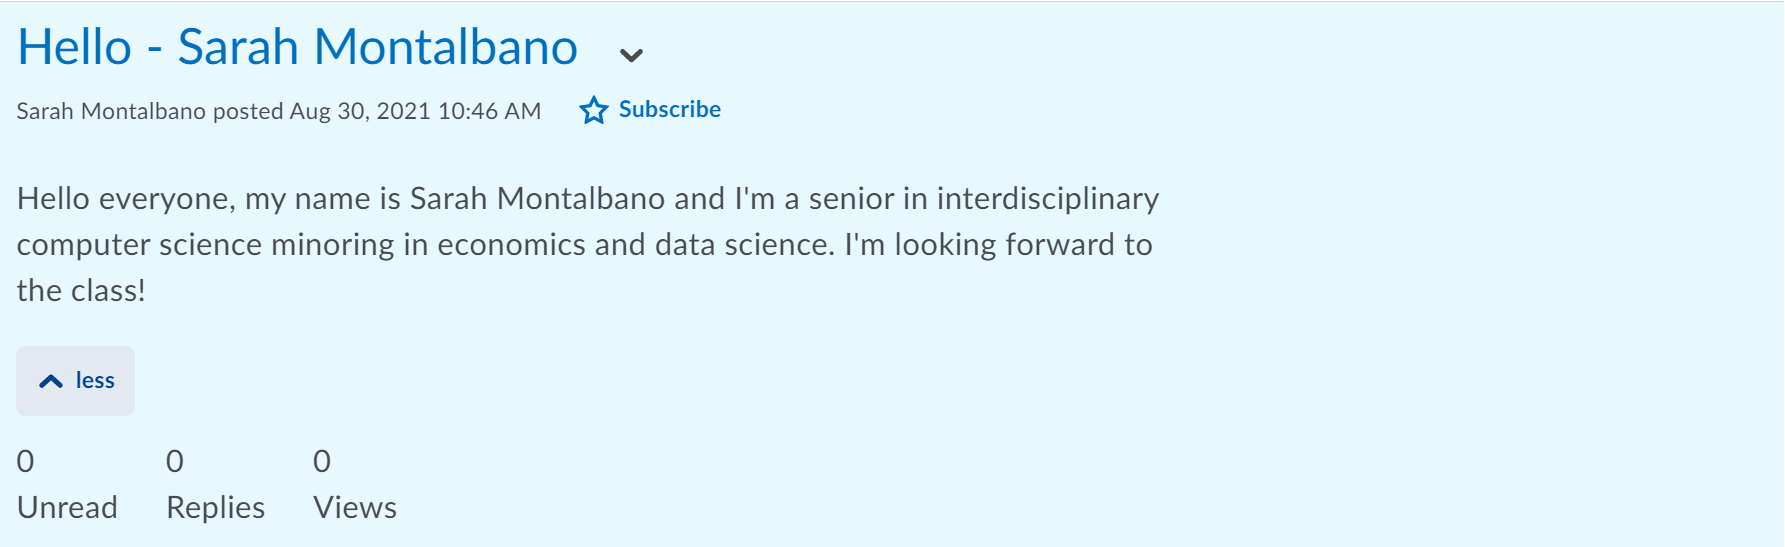
\includegraphics[width=\linewidth]{discussion_board_intro_screenshot.png}
  \caption{My discussion board post on 8-30-2021.}
  \label{fig:screenshot}
\end{figure}

%%%%%%%%%%%%%%%%%%%%%%%%%%%%%%%%%%%%%%%%%%%%%%%%%%%%%%%%%%%%%%%%%%%%%%%%%%%%%%
\collab{None}
\nextprob{Plagiarism}

\begin{enumerate}

    \item In this class, please properly cite all resources that you use. Please
        write your own definition of plagiarism here.  Remember to cite all
        sources!

        \paragraph{Answer}{Plagiarism is the dishonest practice of pretending another person's work is your own. Plagiarism may occur by accident (misquoting, citing wrong source, etc); through self-plagiarism, where a person uses their previous work without proper citation; mosaic plagiarism, using words or phrases from a source without quotation marks or citing; and direct plagiarism, where text is copy and pasted from the source without citation, often without any changes.} 

Citation: 4 types of plagiarism defined here: \url{https://copyleaks.com/blog/types-of-plagiarism}


    \item If you have observed plagiarism or cheating in a classroom (either as
        an instructor or as a student), explain the situation and how it made
        you feel.  If you have not experienced plagiarism or cheating or if you
        would prefer not to reflect on a personal experience, find a news
        article about plagiarism or cheating and explain how you would feel if
        you were one of the people involved.

        \paragraph{Answer}{I was a TA for Honors Texts and Critics last fall and I had a suspicion that one student was not submitting her own work for the take-home essays. The essays often seemed unrelated to the prompt and the style wasn't congruous with her in-class writing; she also put in little effort on other assignments and had admitted to me that she hadn't read the first book on the syllabus. I informed the professor of my concerns, and at the end of the course, recommended that she not receive a passing grade. The professor essentially told me that he knew my concerns and that he would handle assigning final grades. I suspect he passed her but I have no way to know for sure. I was frustrated that my other students, who were doing their assignments by themselves, were going to receive a grade not much better than this student, but I felt powerless to change her behavior after having spoken to her twice before.}
\end{enumerate}

%%%%%%%%%%%%%%%%%%%%%%%%%%%%%%%%%%%%%%%%%%%%%%%%%%%%%%%%%%%%%%%%%%%%%%%%%%%%%%
\collab{None}
\nextprob{Edges in Trees}

Prove or disprove the following statement: Every tree with one or more
nodes/vertices has exactly $n-1$ edges, where $n$ is the number of vertices in
the tree.

\paragraph{Answer}
\begin{proof}{Claim:}{ Every tree with one or more $(n \geq 1)$ nodes/vertices has exactly $n-1$ edges, where $n$ is the number of vertices in the tree.} 
\begin{itemize}
\item \emph{This property will be proved by induction.} 
\item \emph{Base Case:}{ $n = 1$. For $n = 1$, this represents an isolated vertice, and the number of edges must be $n - 1 = 0$.}
\item \emph{Inductive Assumption:}{ Let n = k and assume that the claim is true for k. Any tree with $k$ vertices has $k-1$ edges.}
\item \emph{Inductive Step:}{ For $k \geq 2$. Assume the theorem holds for $k-1$ vertices. Let $T$ be a tree with $k$ vertices, and let $e$ be an edge with end vertices $u$ and $v$. By the definition of a tree, the only path between $u$ and $v$ is $e$. Consider deleting $e$, which results in two disconnected components, $T_1$ and $T_2$, both of which are still trees. The number of total vertices $k$ is the sum of the vertices in $T_1$ and $T_2$, call them $k_1$ and $k_2$. $k_1 + k_2 = k$. Both $k_1$ and $k_2$ must be strictly smaller than $k$.} 
\item \emph{Conclusion:}{ By the induction hypothesis, the number of edges in $T_1$ and $T_2$ are $k_1 - 1$ and $k_2 - 1$. The number of edges in T must be $k_1 - 1$ + $k_2 - 1$ + $1$ = $n_1 + n_2$ - 1 = $n - 1$.}
\end{itemize}
\end{proof}

I consulted \url{http://compalg.inf.elte.hu/~tony/Oktatas/TDK/FINAL/Chap\%204.PDF}, \url{https://www.geeksforgeeks.org/some-theorems-on-trees/}, and \url{http://www.math.ucsd.edu/~gptesler/184a/slides/184a_trees_17-handout.pdf} for examples of proofs on this theorem. For a reminder on induction, I consulted \url{http://web.stanford.edu/class/archive/cs/cs103/cs103.1164/handouts/240\%20Guide\%20to\%20Induction.pdf|}.






%%%%%%%%%%%%%%%%%%%%%%%%%%%%%%%%%%%%%%%%%%%%%%%%%%%%%%%%%%%%%%%%%%%%%%%%%%%%%%
\collab{None}
\nextprob{Big-O}
Use the definition of big-O notation to prove that $f(x)=n^2 + 3n -2$ is
$O(n^2)$.

\paragraph{Answer}
\begin{proof}{Claim:}{$f(x)=n^2 + 3n -2$ is $O(n^2)$.} 
\begin{itemize}
\item \emph{Big-O notation is defined as: $f(x) \leq C\cdot{G(x)}$}
\item { If $f(x)=n^2 + 3n - 2$ is $O(n^2)$, for all $n \geq k$, there exists some constant C such that $n^2 + 3n - 2 \leq C\cdot{n^2}$.}
\item{Suppose $k = 1$, so that $n \geq 1.$ Since $n$ is greater than or equal to 1, $n$ can't be negative and therefore $n^2 \geq n$.}
\item{By the transitive property, $n^2 \geq n \geq 1$. This relation holds true for any multiplication of a constant, like the middle term ($3n^2 \geq 3n \geq 3$). It's also true that $-2n^2 \leq -2n \leq -2.$}
\item{By the previous step, the following inequality is true. $n^2 + 3n - 2 \leq n^2 + 3n^2 - 2n^2.$ Simplifying the right side yields $n^2 + 3n - 2 \leq 2n^2.$}
\item{In conclusion, there exists some constant C such that $C$ ($C = 2$) for all $n \geq = 1$, proving that $f(x)=n^2 + 3n -2$ is $O(n^2)$.}
\end{itemize}
\end{proof}

I consulted \url{https://web.mit.edu/16.070/www/lecture/big_o.pdf} for the mathematical definition of Big-O notation. 

%%%%%%%%%%%%%%%%%%%%%%%%%%%%%%%%%%%%%%%%%%%%%%%%%%%%%%%%%%%%%%%%%%%%%%%%%%%%%%
\collab{None}
\nextprob{If/Then Statements}
Consider the following statement: If $a$ and $b$ are both even numbers, then $ab$ is
an even number.
\begin{enumerate}
    \item What is the definition of an odd number?

        \paragraph{Answer}{An odd number is an integer $n$ such that $n = 2k + 1$, where $k$ is some integer.}

    \item What is the definition of an even number?

        \paragraph{Answer}{An even number is an integer $n$ such that $n = 2k$, where $k$ is some integer.}

    \item What is the contrapositive of this statement?

        \paragraph{Answer}{A contrapositive is, "If not q, then not p." The contrapositive of "If $a$ and $b$ are both even numbers, then $ab$ is an even number" would be, "If either $a$ or $b$ is \textbf{not} an even number, then $ab$ is \textbf{not} an even number."}

    \item What is the converse of this statement?

        \paragraph{Answer}{A converse is, "If q, then p." The converse is, "If $ab$ is an even number, then $a$ and $b$ are both even numbers."}

    \item Prove this statement.

        \paragraph{Answer}{Both $a$ and $b$ are even numbers, which by definition means $a = 2m$ and $b = 2n$, where $m$ and $n$ are some integers. Substituting the definitions of $a$ and $b$, $ab = (2m)(2n) = 4mn$. Since 4 is divisible by 2 and therefore itself even number, we can split into $ab = 2(2mn)$. Let $k = 2mn$. In conclusion, $ab = 2k$, the definition of an even number.}

\end{enumerate}



%%%%%%%%%%%%%%%%%%%%%%%%%%%%%%%%%%%%%%%%%%%%%%%%%%%%%%%%%%%%%%%%%%%%%%%%%%%%%%
\collab{None}
\nextprob{Sorting}
Consider your favorite sorting algorithm.
\begin{enumerate}
    \item \emph{What} is the problem that this algorithm solves?

        \paragraph{Answer}{The collator was invented in 1938, and according to Donald Knuth's The Art of Computer Programming Vol 3, "with its two feeding stations, it could merge two sorted decks of cards into one, in only one pass." Von Neumann designed mergesort, applying the logic of physical card-sorting machines to burgeoning computer science. Mergesort takes a list input and outputs a sorted list. Mergesort has a faster worst-case runtime than most sorting algorithms, works well on large and small datasets, and is especially suitable for linked list problems. Mergesort requires additional memory space, so is not suitable when memory is constrained.}
\\Citation (there's surprisingly little on how mergesort was developed): \url{https://hsm.stackexchange.com/questions/12549/how-did-von-neumann-come-up-with-his-merge-sort-algorithm}

    \item \emph{How} does it work? (Hint: give pseudocode!)

        \paragraph{Answer}
        \begin{algorithmic}
	\Function{MergeSort}{list k} 
	\If {length of $k \leq 1$} \Comment{The base case; a list of length 0 or 1 is trivially sorted.}
	    \State \Return $k$
	\EndIf
	\State left := empty list
	\State right := empty list
	\For {each element of $k$ indexed by $i$}
	\If {$i <$ (length of $k$)/2}
	\State add x to left
	\Else
	\State add x to right
	\EndIf
	\EndFor
	\State left := MergeSort(left)
	\State right := MergeSort(right)
	\State \Return merge(left,right)
	\EndFunction
	\\
	\Function{merge}{left,right}
	\State var result := empty list
	\While {length(left) $>$ 0 and length(right) $>$ 0}
	\If {first(left) $\leq$ first(right)}
	\State{append first(left) to result}
	\State{left := rest(left)}
	\Else
	\State append first(right) to result
	\State right := rest(right)
	\EndIf
	\EndWhile
	\While {left is not empty}
	\State{append first(left) to result}
	\State{left := rest(left)}
	\EndWhile
	\While{right is not empty}
	\State{append first(right) to result}
	\State{right := rest(right)}
	\EndWhile
	\State \Return result
	\EndFunction 
	\end{algorithmic}

Citation: \url{https://www.cs.umd.edu/users/meesh/cmsc351/mount/lectures/lect6-divide-conquer-mergesort.pdf}

    \item \emph{How fast} does it work?  Give the asymptotic running time.
        Note: typically, you will give this as the worst-case running time.
        However, if you chose quicksort or another randomized algorithm, please
        give both the worst-case running time and the expected running time.  No
        justification of the running time is needed.

        \paragraph{Answer}{Mergesort's worst-case performance is $O(n\log{}n)$, which happens to match its best and average-case performance runtimes.}

    \item \emph{Why} does this work? Typically, this will be given as a loop
        invariant proof.  For this HW, explain why it works informally, in your
        own words.

        \paragraph{Answer}{The main function (that breaks down the original list $k$ into the trivially sorted lists of length 1) is correct so long as it distributes the lists of length 1 into different memory and doesn't overwrite. The function that merges and sorts the trivially sorted lists is correct because the nonempty parts of the "result" list always contains the smallest elements of "left" and "right" lists in sorted order. The smallest remaining elements are always at the start of the "left" and "right" lists. So when the algorithm pulls the starting elements of the "left" and "right" lists, it's always taking the smallest elements and sorting them. At the end of copying, the whole list is completely sorted.}
\\Citation: I was curious what a loop invariant would look like for mergesort, so here are some references. It's very above my head for now, but helpful to think harder about merge: \url{http://web.stanford.edu/class/archive/cs/cs161/cs161.1176/Sections/161-section-1.pdf}, \url{https://www.cs.mcgill.ca/~dprecup/courses/IntroCS/Lectures/comp250-lecture16.pdf}.

\end{enumerate}

Note: in all future HWs, if you are asked to come up with an algorithm, you are
expected to give an algorithm that beats the brute force (and, if possible, of
optimal time complexity). With your algorithm, please provide the following:
\begin{itemize}
    \item \emph{What}: A prose explanation of the problem and the algorithm,
        including a description of the input/output.
    \item \emph{How}: Psuedocode, referenced from within the prose explanation.
    \item \emph{How Fast}: Runtime, along with justification.  (Or, in the
        extreme, a proof of termination).
    \item \emph{Why}: Statement of the loop invariant for each loop.
\end{itemize}

\end{document}
